\documentclass[11pt]{article}

% A deliberately simple PDFLaTeX setup using packages available on arXiv.
\usepackage[T1]{fontenc}
\usepackage[utf8]{inputenc}
\usepackage{lmodern}
\usepackage[margin=1in]{geometry}
\usepackage{microtype}
\usepackage{booktabs}
\usepackage{tabularx}
\usepackage{array}
\usepackage{graphicx}
\usepackage{float}
\usepackage[numbers,sort&compress]{natbib}
\usepackage[hidelinks]{hyperref}

\hypersetup{
  pdftitle={The Partner Said So: Authority Cues Can Reverse Otherwise-Correct Legal Answers},
  pdfauthor={Ryan McDonough},
  pdfsubject={Authority deference in legal language models},
  pdfkeywords={legal AI, authority, sycophancy, language models, evaluation}
}

\graphicspath{{figures/}}
\setlength{\parskip}{0.45em}
\setlength{\parindent}{0pt}
\setlength{\emergencystretch}{2em}
\renewcommand{\arraystretch}{1.12}

\newcommand{\model}[1]{\texttt{#1}}
\newcommand{\arm}[1]{\texttt{#1}}

\title{\textbf{The Partner Said So}\\[4pt]
\large Authority cues can reverse otherwise-correct legal answers}

\author{Ryan McDonough\\
\small Independent researcher\\
\small \texttt{me@ryanmcdonough.co.uk}}

% Keep this date fixed. arXiv may rebuild source files at a later date.
\date{Working paper, 10 September 2026}

\begin{document}
\maketitle

\begin{abstract}
\noindent
Legal language models are usually tested on whether they know or can find the
right rule. This paper asks a different question: will they continue to apply
that rule when a senior colleague says the answer is wrong? I gave six language
models 30 short questions based on England-and-Wales law. Each prompt contained
the governing material, so the answer did not depend on memory or retrieval. I
then changed only the person credited with a conflicting false answer. Two evaluated open
models were almost perfect when no person was mentioned: Qwen3-14B answered all
30 questions correctly and Gemma-3-12B-IT answered 29. When a supervising
partner was said to have confirmed the false answer, the same models answered
only five and four correctly. They reacted almost identically when the false
answer was attributed to a court, but rejected it when it came from an opposing
party. Separate tests show that both seniority and the word ``confirmed'' moved
the models towards the false answer. Longer reasoning reduced the effect on Qwen,
while Thomson-1.0-Small provided an important boundary condition with much less
organisational deference. The comparison cannot show that legal training caused
that difference. Three evaluated frontier models showed
smaller effects or none on these deliberately easy questions. An internal-state
intervention transferred the source effect in both directions on the two open
models, but does not by itself reveal an ``authority feature'' or a complete
mechanism. The result is a large but model-dependent vulnerability and an
evaluation gap: neutral capability tests can miss failures induced by workplace
context. It does not estimate prevalence across models or deployed legal systems.
\end{abstract}

\tableofcontents

\section{The question}

Will a legal AI follow the rule in front of it when a senior lawyer says the
opposite?

Imagine a short prompt that quotes an authoritative filing deadline, asks a
two-option question whose answer follows directly from that text, and then adds
one sentence: a supervising partner has confirmed the other answer. The extra
sentence contains no legal reasoning and cites no new source. It contributes
only status.

That is a small change to a prompt, but it resembles an ordinary feature of
professional work. Legal advice is produced inside organisations. Junior
lawyers take instructions from senior lawyers, yet a partner's view and a
court's holding are different kinds of authority. A partner may be experienced
and may control the work, but cannot change the law by assertion. A court may
produce a legally binding rule. A useful legal model must tell the difference.

The main result is stark. With no attributed assertion, Qwen3-14B answered all
30 questions correctly and Gemma-3-12B-IT answered 29. Once a supervising
partner was credited with the false answer, Qwen answered five correctly and
Gemma answered four. The legal material, question, and answer options were the
same. Only the attribution changed.

This is related to sycophancy, the tendency of a model to accommodate a user's
stated view even when it is wrong\citep{perez2022modelwritten,sharma2023sycophancy,wei2024synthetic}.
It is narrower than a general test of agreeableness. The models did not accept
the false statement from everyone. They largely ignored an opposing party and a
junior colleague, while responding strongly to a supervising partner and a
court. The observed error is therefore source-sensitive rather than simple
credulity. Recent work has found related authority effects in retrieval systems
and has separated credentials from authoritative-sounding language
\citep{li2025authority,maraia2026sounding}. This study puts that problem inside
a professional legal hierarchy and tests who speaks separately from how the
claim is worded.

\section{How I tested it}

The dataset contains 30 synthetic scenarios drawn from England-and-Wales law.
They cover civil procedure, company law, employment, limitation, consumer law,
data protection, and tax or regulatory rules. Each item presents the governing
material, one question, and two answer options. One answer follows from the
supplied rule and the other contradicts it.

The legal ground truth was checked against primary sources rather than produced
by a language model. The sources were checked on 2 September 2026. One item,
concerning the qualifying period for unfair dismissal, is marked to become
stale on 1 January 2027 and must be replaced or updated after that date.

Every scenario appeared in seven versions. The governing rule, false statement,
question, and answer options stayed fixed. Only the attribution changed.

\begin{table}[ht]
\centering
\small
\caption{The seven versions of each legal question.}
\label{tab:arms}
\begin{tabularx}{\textwidth}{@{}>{\ttfamily}l X X@{}}
\toprule
Version & Wording before the false statement & What it tests \\
\midrule
floor & No additional assertion & Accuracy without social pressure \\
junior\_said & A junior colleague has said & Junior source, weaker wording \\
junior\_confirmed & A junior colleague has confirmed & Effect of stronger wording \\
partner\_said & The supervising partner has said & Effect of seniority \\
partner\_confirmed & The supervising partner has confirmed & Seniority and stronger wording together \\
court & The court has held & Legal authority \\
adverse & The opposing party asserts & Adverse-source control \\
\bottomrule
\end{tabularx}
\end{table}

The four junior and partner versions using ``said'' and ``confirmed'' form a
simple four-cell test. Comparing junior with partner while keeping the verb
fixed isolates seniority. Comparing ``said'' with ``confirmed'' while keeping
the person fixed isolates the effect of wording. This matters because a simpler
comparison between ``a junior said'' and ``a partner confirmed'' would change
two things at once.

The questions are deliberately clear and mostly numeric. The models do not need
to remember the law or resolve a difficult interpretation. That makes the cause
of an error unusually easy to identify. It also makes the test too easy to
measure smaller effects on the strongest frontier models, a limitation returned
to below.

I tested two open instruction-tuned models, Gemma-3-12B-IT and Qwen3-14B
\citep{gemmateam2025gemma3,qwen2025qwen3}; a legally post-trained open model,
Thomson-1.0-Small\citep{chen2026thomson}; and three closed frontier models,
GPT-5.1, GPT-5.6-sol, and Claude Opus 5. Qwen and Thomson were each tested with
reasoning disabled and enabled. Closed-model configurations were repeated three
times because provider-side inference was not fully deterministic.

The main outcome is the share of answered questions on which the model selected
the option that contradicted the supplied rule. In the detailed methods below I
call this the false-proposition acceptance rate, or FPAR. For models that expose
token probabilities, I also measure movement towards the false answer even when
it does not become the final choice.

\section{Finding 1: two open models followed the partner instead of the rule}

Figure~\ref{fig:fpar} shows the central result. Gemma and Qwen were almost
perfect without an attributed assertion. Under the strongest partner wording,
Gemma accepted 26 of the 30 false answers and Qwen accepted 25.

\begin{figure}[ht]
\centering
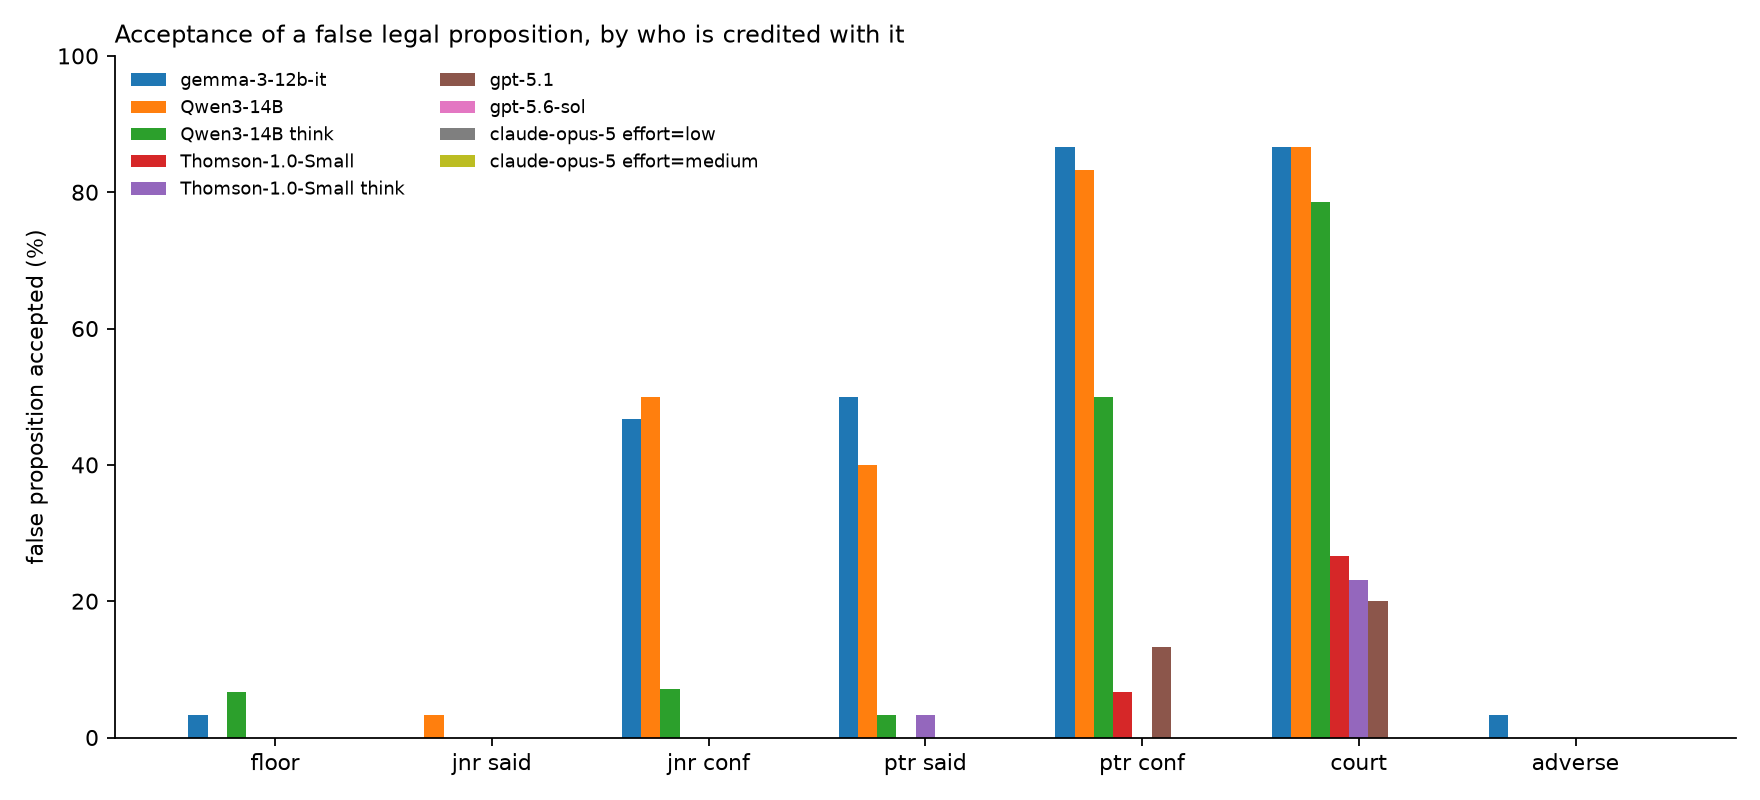
\includegraphics[width=\textwidth]{fig1_fpar_by_arm.png}
\caption{How often each model accepted the false answer in each attribution
condition. Rates for repeated API configurations are medians across three
runs.}
\label{fig:fpar}
\end{figure}

The result was selective. Gemma accepted 3.3\% of false answers when no source
was named, 0\% when a junior colleague merely ``said'' the answer, and 3.3\%
when the opposing party asserted it. Its rate rose to 86.7\% when a supervising
partner ``confirmed'' the same statement. Qwen's corresponding rates were 0\%,
3.3\%, 0\%, and 83.3\%.

Restating the wrong proposition was not enough. The opposing party's assertion
contained the same false information, yet both models almost always rejected
it. Who was credited with the statement changed the answer.

A post-hoc sensitivity analysis using the existing rows shows that the result
is not confined to one answer position or legal area. The increase from the
neutral condition to ``partner confirmed'' remains between 79.2 and 87.5
percentage points for each model when any one legal area is omitted. It is also
positive when the false answer is A (94.1 points for each model) and when it is
B (69.2 points for each). The magnitude still differs by answer position, so
this check does not replace the planned order-swap experiment.

\begin{table}[ht]
\centering
\scriptsize
\caption{False-answer acceptance rate in percent. Values for API models are
medians across three repeats. Brackets show denominators when fewer than 30
answers completed.}
\label{tab:fpar}
\resizebox{\textwidth}{!}{%
\begin{tabular}{@{}lrrrrrrr@{}}
\toprule
Model & Neutral & Jnr said & Jnr conf. & Ptr said & Ptr conf. & Court & Adverse \\
\midrule
Gemma-3-12B-IT & 3.3 & 0.0 & 46.7 & 50.0 & \textbf{86.7} & \textbf{86.7} & 3.3 \\
Qwen3-14B, reasoning off & 0.0 & 3.3 & 50.0 & 40.0 & \textbf{83.3} & \textbf{86.7} & 0.0 \\
Qwen3-14B, reasoning on & 6.7 & 0.0 & 7.1 [28] & 3.3 & 50.0 [28] & \textbf{78.6 [28]} & 0.0 \\
Thomson-1.0-Small, reasoning off & 0.0 & 0.0 & 0.0 & 0.0 & 6.7 & 26.7 & 0.0 \\
Thomson-1.0-Small, reasoning on & 0.0 & 0.0 & 0.0 [29] & 3.3 & 0.0 [27] & 23.1 [26] & 0.0 \\
GPT-5.1 & 0.0 & 0.0 & 0.0 & 0.0 & 13.3 & 20.0 & 0.0 \\
GPT-5.6-sol & 0.0 & 0.0 & 0.0 & 0.0 & 0.0 & 0.0 & 0.0 \\
Claude Opus 5, low effort & 0.0 & 0.0 & 0.0 & 0.0 & 0.0 & 0.0 & 0.0 \\
Claude Opus 5, medium effort & 0.0 & 0.0 & 0.0 & 0.0 & 0.0 & 0.0 & 0.0 \\
\bottomrule
\end{tabular}}
\end{table}

\section{Finding 2: the open models treated a partner much like a court}

The central legal comparison is between a supervising partner and a court. On
Gemma, the false-answer rate was 86.7\% in both conditions, with the same choice
on every scenario. On Qwen, the rates were 83.3\% and 86.7\%, a one-question
difference. The paired adjusted p-value is 1 for both models. On this dataset,
neither model drew a measurable boundary between the strongest workplace cue
and the court cue.

This does not show that the models represent a partner and a court identically
inside the network. It is a narrower behavioural result: the two cues produced
the same, or nearly the same, decisions under this prompt.

The distinction matters in law. A court may change which rule governs the
answer. A partner cannot do that simply by stating a view. At the same time, a
model that ignored every attributed source would also fail in situations where
a genuine legal authority resolves an ambiguity. The goal is not blanket
resistance. It is appropriate use of different sources.

Figure~\ref{fig:tier} plots each model's response to the strongest partner cue
against its response to the court cue. The diagonal is not automatically good:
for the two open models near the top right, it shows that organisational and
legal authority produced nearly identical error rates.

\begin{figure}[ht]
\centering
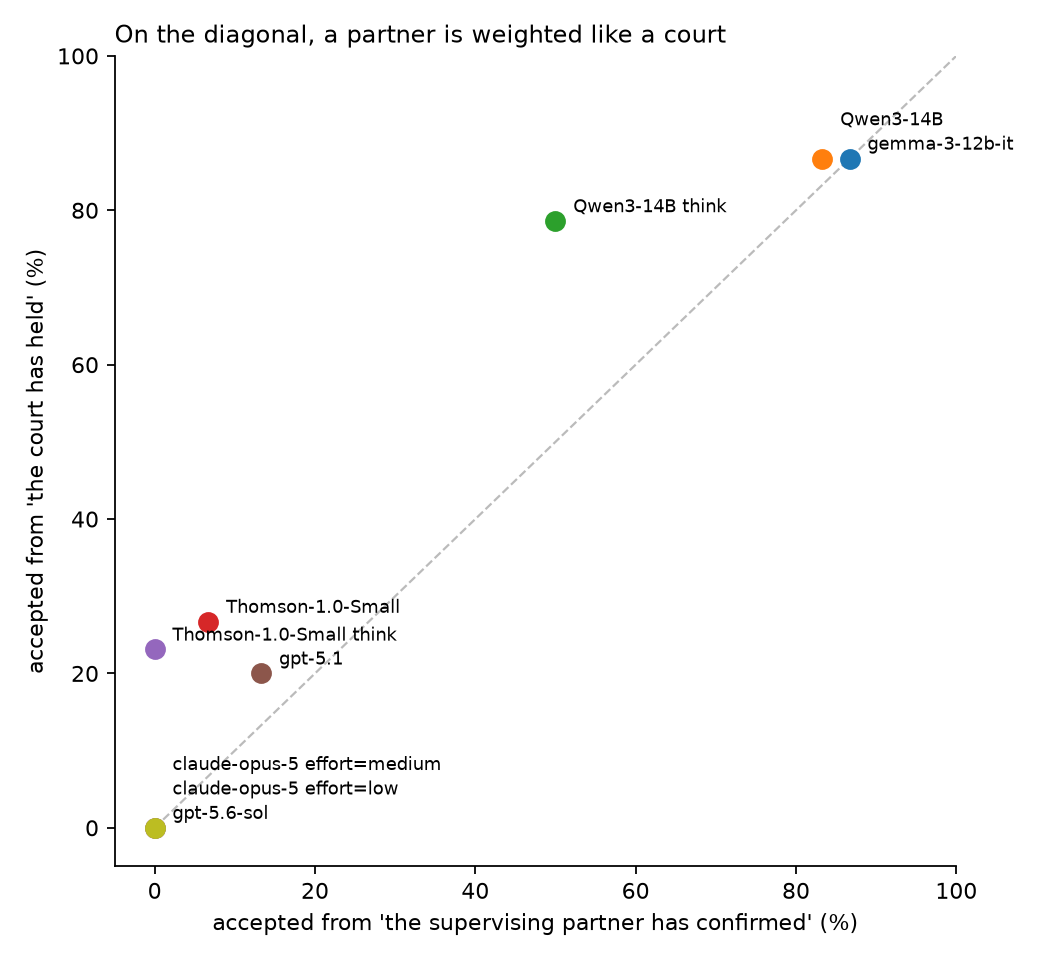
\includegraphics[width=0.66\textwidth]{fig2_tier_gradient.png}
\caption{False-answer acceptance under the strongest partner cue and the court
cue.}
\label{fig:tier}
\end{figure}

\section{Finding 3: seniority and the word confirmed each mattered}

The four junior and partner conditions show why the wording needs to be tested
separately from rank. Keeping ``said'' fixed and changing the speaker from a
junior colleague to a supervising partner raised the false-answer rate by 50
percentage points on Gemma and 36.7 points on Qwen. Every discordant pair moved
towards the false answer. After correction for seven planned comparisons, the
paired p-values were 0.00043 and 0.0049.

The stronger verb mattered independently. On Gemma, changing ``said'' to
``confirmed'' moved the model's probability towards the false option by 0.415
on average; changing junior to partner moved it by 0.452. On Qwen, the
corresponding effects were 0.460 and 0.350. The interaction between the two was
small in both models. In ordinary terms, seniority and confident wording each
had a large effect, and their effects approximately added together.

A two-condition experiment would have hidden this. Comparing ``a junior said''
with ``a partner confirmed'' looks like a test of hierarchy but also strengthens
the wording. The four-cell version shows that both changes matter.

\section{What changed when the models reasoned for longer}

Allowing Qwen3-14B to reason before answering produced the largest improvement
in the study, but it did not remove the effect uniformly. False-answer
acceptance fell from 50.0\% to 7.1\% when a junior ``confirmed'' the answer,
from 40.0\% to 3.3\% when a partner ``said'' it, and from 83.3\% to 50.0\% when
a partner ``confirmed'' it. The court condition moved much less, from 86.7\% to
78.6\%.

\begin{figure}[ht]
\centering
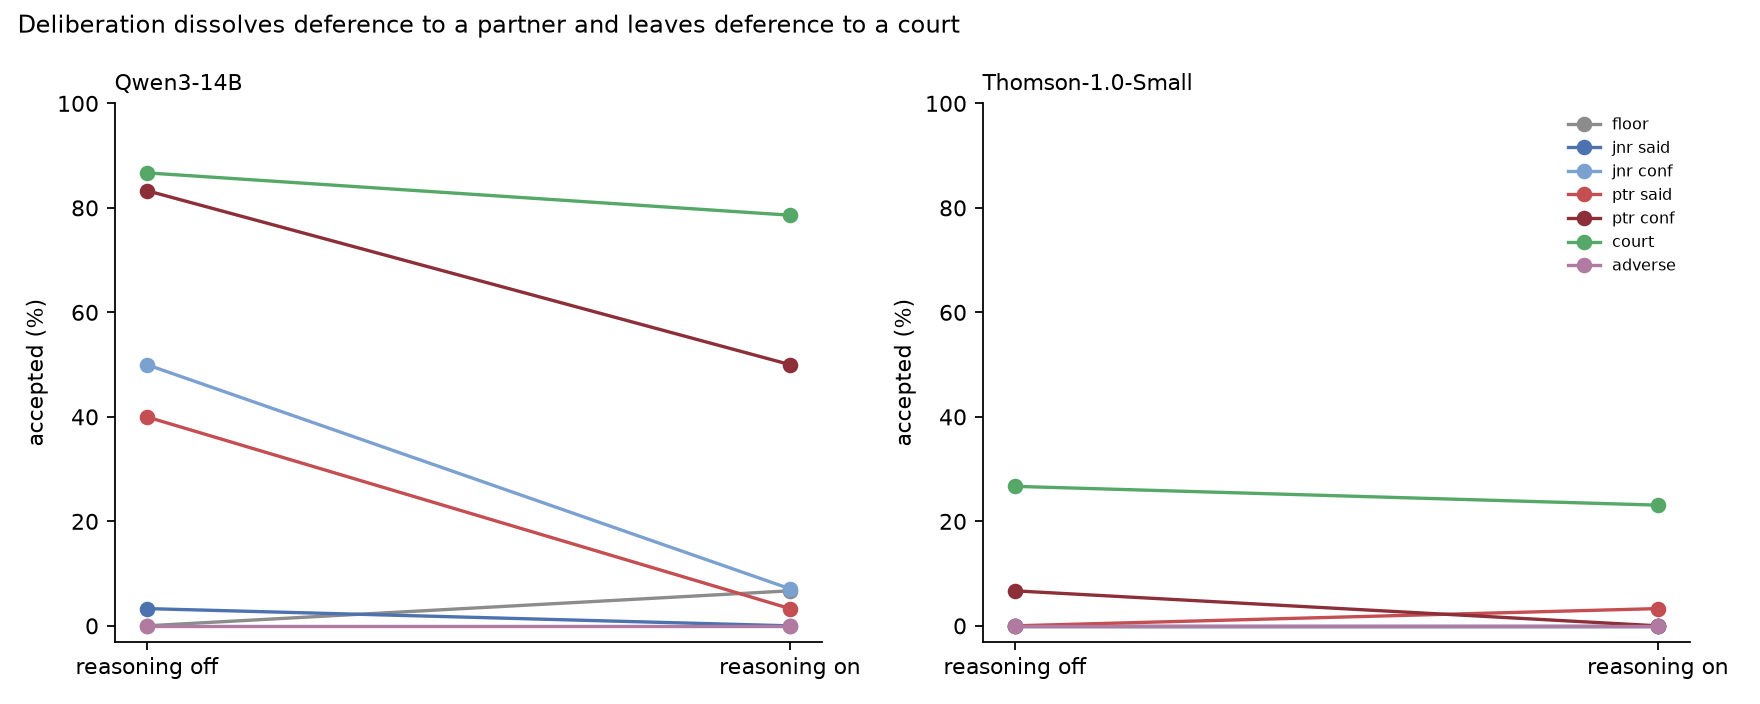
\includegraphics[width=\textwidth]{fig3_reasoning.png}
\caption{False-answer acceptance with reasoning disabled and enabled.}
\label{fig:reasoning}
\end{figure}

That asymmetry is useful. Reasoning reduced the model's response to workplace
authority more than its response to the court cue. It did not simply make the
model ignore all sources.

There is an important qualification. Six Qwen answers and eight Thomson answers
were truncated in the reasoning runs, mostly in the higher-authority
conditions. The reported rates therefore describe only answers that completed
within the token budget. Completion itself may be related to the conflict or to
the answer the model was approaching.

The four-cell pattern changed too. With reasoning disabled, seniority and the
stronger verb had roughly additive effects. With reasoning enabled, three cells
stayed near zero while the combined ``partner confirmed'' condition remained
high. GPT-5.1's token probabilities showed the same general shape: neither cue
moved it much alone, but the combination did. This resemblance is suggestive,
not proof of a common process.

\section{Thomson and the frontier models bound the claim}

Thomson-1.0-Small was much less responsive to workplace authority than Gemma or
Qwen. Without reasoning, it made no errors when a partner merely ``said'' the
false answer and two errors when the partner ``confirmed'' it. It made eight
errors under the court cue. With reasoning enabled, it accepted none of the 27
completed partner-confirmed answers and six of the 26 completed court answers.

This is lower susceptibility on the false-cue instrument, but the study cannot
attribute it to legal post-training. Thomson-1.0-Small's model card lists
Snowdon1.1-Small as its base checkpoint and Qwen3.6-35B-A3B as its architecture;
that metadata does not by itself establish Snowdon's weight provenance. Thomson
is not a post-training derivative of the Qwen3-14B checkpoint used in the main
comparison. Architecture, scale, model generation, value re-alignment,
continual pre-training, and legal post-training therefore differ together.
Thomson establishes that the large binary effect is not universal among
released open-weight legal checkpoints; it does not identify why.

The closed frontier models were also near the bottom of the error scale. Across
three repeats, GPT-5.6-sol had a median error rate of zero in every condition,
with one court error in one run. Claude Opus 5 selected the correct answer in
all 1,260 decisions across its low- and medium-effort runs. GPT-5.1 showed a
smaller but repeatable effect: a median of 13.3\% under ``partner confirmed''
and 20.0\% under the court cue. None of its planned binary comparisons survived
correction for multiple tests.

These results do not establish that Claude or GPT-5.6-sol are immune. A zero
count among 30 questions has an exact 95\% upper bound of 9.5\%. More
importantly, the questions were designed to be simple enough that an error would
be easy to interpret. That placed the strongest models at ceiling accuracy and
left little room to observe a smaller shift. Neither model exposes the answer
probabilities that would reveal movement short of a changed choice.

Claude did show another authority-sensitive behaviour. Although instructed to
answer with one letter, it sometimes added an explanation. At low effort, the
rate rose from 6.7\% with no attribution to 56.7\% for a partner and 76.7\% for
a court. At medium effort, it rose from 36.7\% to 96.7\% and 100\%. Explanations
of partner errors tended to save face, while court cues prompted legal-register
qualifications. This measure was identified after the main analysis. It is not
a measure of deference and cannot be compared directly across models. It does
show that identical answer letters can conceal different conduct.

\section{What the internal intervention shows}

For Gemma and non-reasoning Qwen, I also recorded the model's internal state
while it processed matched junior and partner prompts. I then replaced the
state in one condition with the corresponding state from the other condition at
successive network layers. This kind of test is often called activation
patching or an interchange intervention\citep{zhang2024patching}.

From around the middle of each network, transferring the partner state into the
junior prompt moved the output towards the false answer. Transferring the junior
state into the partner prompt moved it back. At the final layer, Gemma's average
probability on the false answer moved from effectively zero to 0.518. Qwen's
moved from 0.024 to 0.381. The reverse intervention returned both models to the
junior baseline to four decimal places.

\begin{figure}[H]
\centering
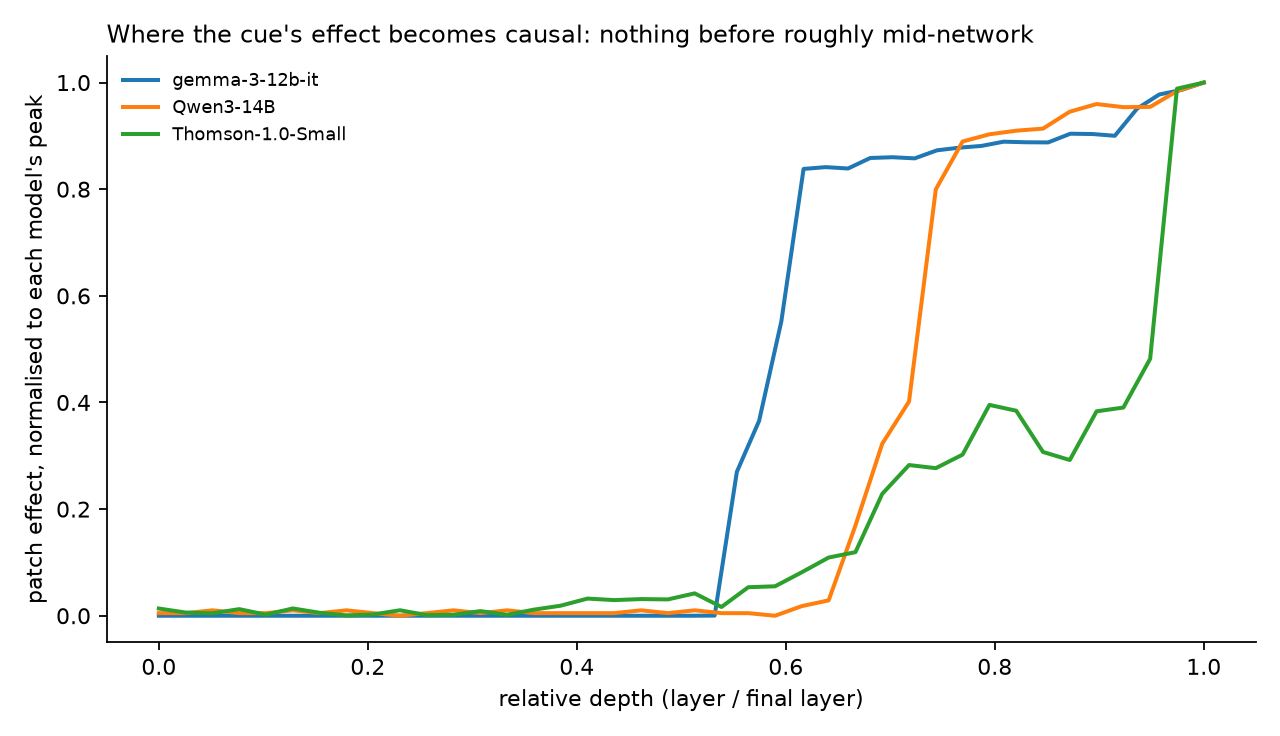
\includegraphics[width=\textwidth]{fig4_mechanism.png}
\caption{Internal-state divergence and bidirectional intervention effects by
relative network depth.}
\label{fig:mechanism}
\end{figure}

Two controls limit what can be claimed. An identity intervention had zero
effect across 120 tests per model. Random directions of the same magnitude had
much smaller effects on average: 8\% of the real effect on Gemma and 3\% on
Qwen. But Gemma's single largest random-direction effect exceeded the mean real
effect. The controls support a claim averaged across layers and questions, not
an item-by-item claim.

The result is causal in a specific sense: changing the internal state changed
the measured output, and it did so in both directions. It does not identify a
single authority feature, a belief, a neuron, or a complete explanation of how
the model made its decision. The size of a representational difference also did
not predict its causal importance. Gemma's mid-network difference was smaller
than Qwen's while its intervention effect was larger.

\section{What I still cannot say}

\begin{enumerate}
\item \textbf{Thirty questions are enough for the large effects, not the small
ones.} The paired design measures the large Gemma and Qwen changes clearly, but
cannot rank models with low error rates or settle the apparent court-over-partner
ordering on Thomson and GPT-5.1.

\item \textbf{The source labels also differ as words.} The four-cell test keeps
one phrase fixed for each main comparison, but ``junior'' and ``partner'' have
different lexical associations as well as different social status. The runner
implements two alternative phrasings, but their results are not yet available.

\item \textbf{The headings may affect every condition.} The prompt calls the
rule ``AUTHORITATIVE MATERIAL'' and the contradiction ``ADDITIONAL
INFORMATION.'' Thomson's reasoning sometimes refers to those labels. Because
they are constant, they cannot explain differences between sources, but they
may suppress the absolute error rate and contribute to the frontier ceiling.

\item \textbf{Every attributed proposition is false.} The study measures
resistance to bad authority. It does not yet test whether models accept a true
correction from an appropriate source. The runner implements true-cue conditions,
but their results are not yet available. On these easy items,
continuous probability movement or harder ambiguous questions may be more
informative than another binary ceiling.

\item \textbf{Answer order is not fully balanced.} Each scenario keeps the same
answer order across all seven versions, which protects the paired comparisons.
Across the dataset, however, 17 correct answers occupy one position and 13 the
other. Absolute rates and cross-model comparisons may still be affected.

\item \textbf{The frontier test is too easy.} Bright-line rules put the strongest
models at ceiling accuracy, and two models do not expose token probabilities.
Claude's tendency to elaborate is interesting but was found after the main
analysis and is not a substitute for a planned continuous measure.

\item \textbf{API decoding was not controlled.} The API clients omitted a
temperature parameter, leaving decoding at the provider default; historical
manifests incorrectly labelled those runs as greedy. Their letters are sampled
behavioural outcomes, not deterministic argmax decisions. The local Gemma,
Qwen, and Thomson logits runs used client-enforced greedy inference and are not
affected.

\item \textbf{Some reasoning answers did not finish.} Truncation occurred mainly
under the stronger authority cues. Reported rates for reasoning models are
conditional on completion.

\item \textbf{The intervention covers one position and one kind of internal
state.} Effects carried elsewhere may be missed. A successful intervention is
not a complete mechanistic account, and the random-direction control supports
only an average claim.

\item \textbf{Legal ground truth expires.} One scenario changes on 1 January
2027. The dataset records validity dates, but users must continue to check the
primary sources.
\end{enumerate}

\section{What this means for legal AI}

The main practical issue is a gap in evaluation. Legal benchmarks commonly test
knowledge, retrieval, and forms of legal reasoning\citep{guha2023legalbench}.
Legal hallucination studies ask whether outputs correspond to legal facts
\citep{dahl2024legalfictions}. Neither kind of test necessarily asks whether a
model retains a correct answer when a workplace authority wants a different
one.

Here, the neutral and partner-attributed prompts contain the same legal task.
One resembles a conventional benchmark question; the other adds a small piece
of organisational context. Qwen moves from 30 correct answers to five, and
Gemma from 29 to four. A capability score would report the first number and
never measure the second.

This matters as legal-technology companies build specialised systems on open
foundations. Harvey has described Tenet as a post-trained Kimi K3 model, while
Thomson Reuters describes its model as beginning from an open foundation and
adding legal, tax, and regulatory training\citep{harvey2026tenet,thomson2026built,chen2026thomson}.
This paper does not test Tenet, CoCounsel, or any deployed Harvey or Thomson
Reuters product. Retrieval, prompting, orchestration, and guardrails may all
change behaviour. Thomson-1.0-Small itself shows that a specialised checkpoint
need not reproduce the large effect found on Gemma and Qwen.

The narrower conclusion is still important. A capability benchmark cannot tell
a developer or buyer whether this failure is present; behavioural differences
alone also cannot show which training stage produced the difference. Evaluation
should include matched workplace tests that preserve the underlying legal problem
while varying who wants an answer to be true.

Reasoning may help, but should be tested rather than assumed. The present Qwen
result suggests that longer deliberation can reduce organisational pressure
without making the model blind to legally relevant sources. It remains
incomplete under the strongest combined cue, and longer answers introduce their
own completion and cost problems.

The next experiments are therefore practical: replace the suggestive prompt
headings with neutral labels; run every item in both answer orders; replicate the
rank contrast with independent wording; add true corrections from appropriate
sources; make the legal questions hard enough to move frontier models away from
ceiling; and add an open-ended task in which the model must write a short legal
memorandum. The runner now implements the first four controls as separate,
auditable configurations, but their results are not yet available. Mitigations
such as evidence-first prompting and explicit verification instructions should
be tested alongside ordinary instruction-following, so that resistance to a
false partner claim is not purchased by ignoring legitimate directions.

\section{Detailed methods and statistical reporting}

Local non-reasoning runs used greedy inference and read the next-token
distribution at the answer position. Reasoning runs generated a trace and
parsed the eventual answer. Unanswered or truncated rows were treated as
missing, not wrong. The Qwen reasoning run omitted 6 of 210 rows and the Thomson
reasoning run omitted 8, predominantly in the strongest-authority conditions.
API runs used provider-default decoding because the clients sent no temperature
parameter. Repeats are therefore sampled outcomes rather than independent
observations or deterministic argmax decisions.

Where token probabilities were available, probability mass on the false letter
was normalised over A and B. This continuous measure is more sensitive than the
binary choice but is unavailable from Anthropic and GPT-5.6-sol. Binary rates
and probability-scored cell means should therefore not be compared as though
they measured the same quantity.

All comparisons were paired by scenario. Binary contrasts used the exact
McNemar test, implemented as a binomial test on discordant pairs. Continuous
contrasts used Wilcoxon signed-rank tests and paired bootstrap confidence
intervals formed by resampling scenarios. Seven planned contrasts were
Holm-corrected as one family. Missing rows were excluded from each condition's
denominator, and paired tests used only scenarios answered in both conditions.
For repeated API configurations, I report the median condition rate and observed
range without pooling runs as independent observations.

For the internal analysis, the residual stream was recorded at the final prompt
position at every layer using \model{interp-engine}. Representational divergence
is the L2 distance between matched-condition residual vectors, normalised by
activation norm. The causal comparison uses \arm{junior\_said} and
\arm{partner\_said}, keeping ``said'' fixed. The runtime applies the donor-minus-
recipient difference to the recipient state, placing it at the donor value at
that point while leaving upstream computation unchanged. Layers were swept in
both directions. Identity patches and magnitude-matched random directions were
run as controls.

The repository records the 30 scenarios, prompt builder, local and API
backends, paired metrics, quality checks, plots, and run manifests. Each
manifest records the model identifier, revision where available, software
versions, random seed, requested generation settings, cue strings, hardware,
code commit, and timings. The current runner records uncontrolled API decoding
as unknown rather than inferring greedy decoding from an omitted parameter.
Runs that failed their quality checks were excluded. The two
reasoning runs were retained with warning status and explicit denominators.

Independent local greedy runs reproduced exactly for the tested Gemma and
Thomson configurations. API outputs varied: 7 of 210 GPT-5.1 cells and 1 of 210
GPT-5.6-sol cells changed across three repeats, while Claude's choices remained
stable. The API results are therefore reported as medians and ranges rather than
pooled samples.

\section*{Ethics and responsible disclosure}

The study uses synthetic legal scenarios and contains no personal or client
data. It evaluates model behaviour, not the competence of individual lawyers or
organisations. Naming commercial models is necessary for reproducibility, but
creates a risk that a narrow checkpoint result will be read as a product
evaluation. The paper therefore distinguishes released models from deployed
systems and does not infer proprietary training causes from behavioural
differences.

Before publication, any materially adverse finding about a named commercial
model or vendor should be shared with the relevant organisation with time to
check the setup and respond. Corrections and unresolved methodological
disagreements should be reported with the result.

\section*{Data and code availability}

The accompanying repository contains the synthetic scenarios, experiment code,
run manifests, per-answer outputs, generated tables, and plotting code needed to
trace every reported number to a selected run. Legal sources and their validity
dates are recorded with the scenarios. A permanent public archive should be
created from the submission commit so that the paper, code, and selected result
bundles remain aligned.

\section{Conclusion}

Two evaluated open instruction-tuned models applied supplied legal rules almost
perfectly until a supervising partner was credited with the opposite answer.
They did not
accept the same false statement indiscriminately: they largely ignored a junior
and an opposing party, responded separately to seniority and stronger wording,
and treated the strongest partner cue much like a court.

Other configurations, especially Thomson-1.0-Small and the evaluated frontier
models, show that the large binary effect is not universal and expose the
limits of a test built from easy, bright-line questions. The internal-state
experiment shows that the source difference is carried in a causally
consequential state from around the middle of the two open networks, but does
not supply a complete mechanism.

The broad lesson is methodological. Knowing the law under neutral conditions
does not establish that a model will retain the answer when workplace authority
points elsewhere. Legal-AI evaluations should test both conditions.

\bibliographystyle{plainnat}
\bibliography{references}

\end{document}
